\documentclass{ximera}

\newcommand{\RR}{\mathbb R}
\renewcommand{\d}{\,d}
\newcommand{\dd}[2][]{\frac{d #1}{d #2}}
\renewcommand{\l}{\ell}
\newcommand{\ddx}{\frac{d}{dx}}
\newcommand{\dfn}{\textbf}
\newcommand{\eval}[1]{\bigg[ #1 \bigg]}


\author{Jim Talamo}
\license{Creative Commons 3.0 By-NC}


\outcome{Review integration techniques}


\begin{document}
\begin{exercise}
When solving separable equations, any integration technique may be necessary to evaluate antiderivatives.  This exercise reviews a few of the ones we've seen already.

\begin{exercise}
Use integration by parts to determine the integral:
\[
\int (2x-6) e^{8x} \d x 
\]


Choose $u=\answer{ 2x-6}$ and $\d v=\answer{e^{8x} } \d x$. 

Then $\d u= \answer{ 2 } \d x$ and $v= \answer{ \frac{e^{8x}}{8} }$.

Using the integration by parts formula, we obtain:

\[
\int (2x-6)e^{8x} \d x= \answer{(2x-6)\frac{e^{8x}}{8}} - \int \answer{ \frac{e^{8x}}{4} } \d x
\]

Calculating the right hand side we obtain

\[
\int (2x-6)e^{8x} \d x= \answer{ (2x-6)\frac{e^{8x}}{8} - \frac{e^{8x}}{32} +C}
\]
(Use $C$ for the constant of integration)
\end{exercise}
%%%%%%%%%%%%%%%%%%%%%%%%%%%%%%%%%%%%%
\begin{exercise}
Determine the integral
\[
\int \cos^{4}(x) \sin^{5}(x) \d x
\]

We should let $u=\answer{\cos(x)}$ so $\d u= \answer{ -\sin(x)} \d x$. 

Rewriting our integral in terms of $u$ we obtain: 

\[
\int \answer{ -u^{4} (1-u^{2})^{2} }\d u
\]

Integrating and then substituting back for $x$ we have:

\[
\int \cos^{4}(x) \sin^{5}(x) \d x=\answer{- \left( \frac{ \cos^{5}(x)}{5} + \frac{ \cos^{9}(x)}{9} -\frac{2 \cos^{7}(x)}{7} \right)+C }
\]
(Use $C$ for the constant of integration)
\end{exercise}
%%%%%%%%%%%%%%%%%%%%%%%%%%%%%%%%%%%%%
\begin{exercise}
Use trigonometric substitution to determine the integral.
\[
\int 50 x^{3} \sqrt{1-25x^{2}} \d x
\]

First we must determine the appropriate substitution. 

Since we have a $1-25x^{2}$ term, we should use $x=\answer{\frac{1}{5}\sin(\theta)}$. 

This means that $\d x= \answer{\frac{1}{5}\cos(\theta)} \d \theta$. 

\begin{exercise}
Using the trig identity $1-\sin^{2}(\theta)=\cos^{2}(\theta)$, we can rewrite $1-25x^{2}$ as $\answer{\cos^{2}(\theta)}$. 

Now we can express our original integral as a trigonometric integral in terms of the variable $\theta$. 

\[
\int  50 x^{3} \sqrt{1-25x^{2}} \d x= \int \answer{  \frac{2}{25} \sin^{3}(\theta) \cos^{2}(\theta)  } \d \theta\
\]

This is a trigonometric integral that can be evaluated easily by using the substitution $u = \answer{\cos(\theta)}$.  Carrying out the details, the antiderivative in terms of $\theta$ is: 

\[
\int \frac{2}{25} \sin^{3}(\theta) \cos^{2}(\theta)   \d \theta\ = \answer{ \frac{-2}{25}\left( \frac{\cos^{3}(\theta)}{3} -\frac{\cos^{5}(\theta)}{5} \right) + C}
\]
(Use $C$ for the constant of integration)


Now we really want the antiderivate in terms of $x$ since our functions was originally in terms of $x$. 

\begin{exercise}
Using the original substitution $x=\frac{1}{5}\sin(\theta)$, we draw the right triangle 

    \begin{image}
      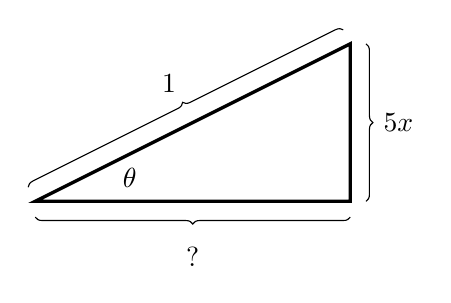
\begin{tikzpicture}
        \coordinate (C) at (0,2);
        \coordinate (D) at (4,2);
        \coordinate (E) at (4,4);
        \tkzMarkRightAngle(C,D,E)
        \tkzMarkAngle(D,C,E)
        \draw[decoration={brace,mirror,raise=.2cm},decorate,thin] (0,2)--(4,2);
        \draw[decoration={brace,mirror,raise=.2cm},decorate,thin] (4,2)--(4,4);
        \draw[decoration={brace,raise=.2cm},decorate,thin] (0,2)--(4,4);
        \draw[very thick] (D)--(E)--(C)--cycle;
        \node at (2,2-.7) {$?$}; %% adj
        \node[anchor=west] at (4+.3,3) {$5x$}; %% opp 
        \node at (2-.3,3+.5) {$1$}; %% hyp
        \node at (1.2,2.3) {$\theta$};
      \end{tikzpicture}
    \end{image}

Then using the Pythagorean Theorem we find that the
 length of the side adjacent to $\theta$ is $\answer{\sqrt{1-25x^{2}}}$. 

Using the triangle, we now convert each of the expressions in our antiderivative that was in terms of $\theta$ to be in terms of $x$:

\[
\cos(\theta)=\answer{\sqrt{1-25x^{2}}}
\]

\begin{exercise}
Hence the answer to our original integral is: 

\[
\int 50 x^{3} \sqrt{1-25x^{2}}  \d x= \answer{ \frac{-2}{25} \left( \frac{1}{3}(1-25x^{2})^{\frac{3}{2}} - \frac{1}{5}(1-25x^{2})^{\frac{5}{2}}\right) + C }
\]
(Use $C$ for the constant of integration)
%%%%%%%%%%%%%%%%%%%%%%%%%%%%%%%%%%%%%
\begin{exercise}
Use the method of partial fractions to determine the integral.
\[
\int \frac{2x-8}{x^2+8x+12} \d x
\]

We must decompose the rational function into simpler rational pieces which we can integrate. 
Note that the degree of the numerator is smaller than the degree of the denominator so we do not need 
to use long division. 

First we see if we can factor the denominator. 

In this case we can factor and we get:
\[
x^{2}+8x+12=(x+6)(x+2)
\]

That means, for some constants $A$ and $B$, we have:

\[
\frac{2x-8}{x^{2}+8x+12}= \frac{A}{x+6} + \frac{B}{x+2}
\]

We need to determine the constants $A$ and $B$. 

We clear denominators by multiplying both sides of the above equation by $\answer{(x+6)(x+2)}$. 

This gives us 

\[
2x-8=A(x+2) + B(x+6)
\]

We can determine the unknown coefficients $A$ and $B$ in two ways. 
We could expand the right hand side and then identify coefficients of like terms on the left and right.
Instead, for this case, we try certain convenient values of $x$ to simplify the above equation and then solve for the coefficients. 

Let us try plugging in $x=-2$ into the above equation. 

Then we get 
\[
\answer{-12 }= B\answer{4}
\]

This tells us that $B=\answer{ -3}$. 


In a similar fashion we can plug in $x=-6$. 

Then we have 

\[
\answer{-20}=A\answer{-4}
\]

Solving, we obtain $A=\answer{5}$. 

\begin{exercise}
This means our original integral can be rewritten as 

\[
\int \frac{2x-8}{x^{2}+8x+12} \d x= \int \frac{5}{x+6} \d x + \int \frac{-3}{x+2} \d x
\]

 Finally computing the antiderivative we get 

\[
\int \frac{2x-8}{x^{2}+8x+12} \d x= \answer{ 5\ln|x+6|-3\ln|x+2| + C }
\]
(Use $C$ for the constant of integration)

\end{exercise}
\end{exercise}
\end{exercise}
\end{exercise}
\end{exercise}
\end{exercise}
%%%%%%%%%%%%%%%%%%%%%%%%%%%%%%%%%%%%%


\end{exercise}
\end{document}
